\section{Introduction}
\label{section_search_intro}
In the previous chapters we have laid the groundwork for the main event: searching for new asteroids in the ZTF dataset.
Here is an outline of the search process, which will be elaborated in greater detail in the sections below.
The search is initialized with a set of candidate orbital elements that is generated randomly based on the orbital elements of known asteroids.
The orbits are integrated over the unique times present in the ZTF data, 
and the subset of ZTF detections within a threshold (2 degrees) of each candidate element is assembled.

A custom Keras Model class called \tty{AsteroidSearch} performs a search using gradient descent.
This search optimizes an objective function that is closely related to the joint log likelihood of the orbital elements
as well a set of parameters describing a mixture model.
The mixture model describes the probability distribution of the squared relative distance over the threshold, $v$, as a mixture of hits and misses.
Hits are modeled as following an exponential distribution, and misses are modeled as being distributed uniformly.
A set schedule of adaptive training is run.  
This training schedule has alternating periods of training just the mixture parameters at a high learning rate
and jointly training the mixture parameters and orbital elements.

At the conclusion of the training process, we tabulate ``hits'' which are here defined as ZTF detections that are within 10 arc seconds of the predicted direction.
All the fitted orbital elements are saved along with summary statistics of how well they were fit including the mixture parameters.
The most important indicator is the number of hits.
Candidate orbital elements with at least 5 hits are deemed noteworthy and candidates with 8 or more hits are deemed to have been provisionally fit.
The search program also saves the ZTF detections associated with each fitted orbital element.

I demonstrate the effectiveness of this method in a series of increasingly difficult tests.  
The easier tests involve recovering the orbital elements of known asteroids that have many hits in the ZTF dataset.
The most difficult task is to identify the orbital elements of new asteroids by searching the subset of ZTF detections that don't match the known asteroid catalogue.
In particular, the five tasks presented are
\begin{itemize}
\item recover the elements of known asteroids starting with the exact elements, but uninformed mixture parameters
\item recover the elements of known asteroids starting with lightly perturbed elements
\item recover the elements of known asteroids starting with heavily perturbed elements
\item ``rediscover'' the elements of known asteroids starting with randomly initialized elements
\item discover the elements of unknown asteroids starting with randomly initialized elements
\end{itemize}
The search process presented passes the first three test with varying degrees of success, 
recovering 64, 42 and 12 elements, respectively, out of the 64 candidates.
The search for known asteroids from random initializations has 1 success on the first batch of 64 and is eventually run on a large scale,
where it plausibly recovers elements of 125 known asteroids.
The search for previously unknown asteroids yields 9 candidate orbital elements that I claim 
might plausibly belong to real but uncatalogued asteroids.

I tested the quality of the results by comparing the fitted orbital elements to the known orbital elements on two metrics.
The most important indicator is to compare the orbits on a set of representative dates and compute the mean squared difference in the position in AU.
A secondary metric is to compare the orbital elements themselves.  
This is done with a metric that standardizes each element and assigns it an importance score.
Both of these metrics show excellent agreement of the recovered orbital elements with the existing elements in the asteroid catalogue.

\section{Generating Candidate Orbital Elements}
\label{section_candidate_elements}
The search is initialized with a batch of candidate orbital elements. 
The batch size is a programming detail; I selected $n=64$.
The choice of initial orbital elements is critically important to the search.
Unlike with other problems, where in theory there is often one globally correct answer 
that might or might not be reachable depending on the initialization, 
the number of local maxima in the objective function here will be at least the number of real asteroids adequately represented in the data.
Based on the last chapter, that means there are over 100,000 local maxima in the objective function.

In this work, I use a simple strategy of random initializations.
Improving on this initialization strategy is the most important item of future work.
I had originally planned to upgrade this to a more intelligent initialization but unfortunately ran out of time.
Random initialization would be nearly hopeless if we had no information about the probability distribution of orbital elements.
But because we have access to large asteroid catalogue, it is feasible to generate plausible candidate elements.

The random initialization strategy breaks the six orbital elements into two categories: empirical and uniform.
The elements $a$, $e$, $i$ and $\Omega$ are sampled from the empirical distribution.
To be more precise, four random indices $j_{a}$, $j_{e}$, $j_{i}$ and $j_{\Omega}$ between 1 and 733,489 are selected, 
and the initialization is done by setting e.g. $a_{j}$ equal to the semi-major axis of the known asteroid with number $j_{a}$.
The two orbital elements $M$ and $\omega$ are initialized uniformly at random on the interval $[0, 2\pi)$.
We know from Kepler's second law (equal time in equal area) that the mean anomaly $M$ is linear in time,
so we have a solid theoretical argument for sampling it uniformly.
Once $M$ is determined, it is converted to $f$ using \tty{REBOUND}.
I will show empirically that the argument of perihelion $\omega$ appears to be distributed very close to uniformly as well.

Figures ~\ref{fig:elt_dist_a}, ~\ref{fig:elt_dist_e_i}, and ~\ref{fig:elt_dist_Omega_f} plot PDFs 
for selected mathematical transformations of orbital elements.
\begin{figure}[hbt!]
\begin{center}
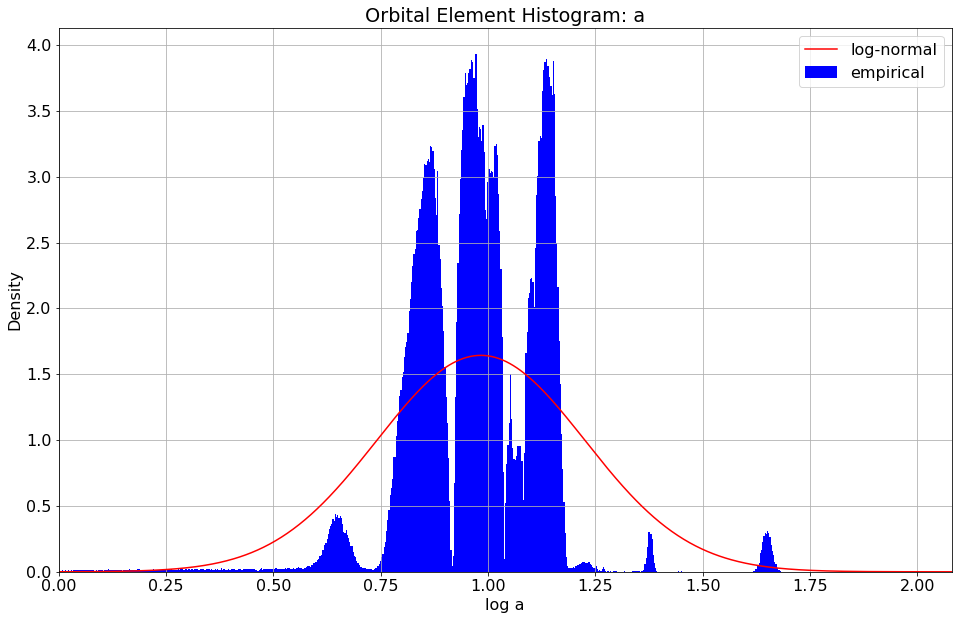
\includegraphics[width=1.0\textwidth]{../figs/elts/elt_hist_a_pdf.png}
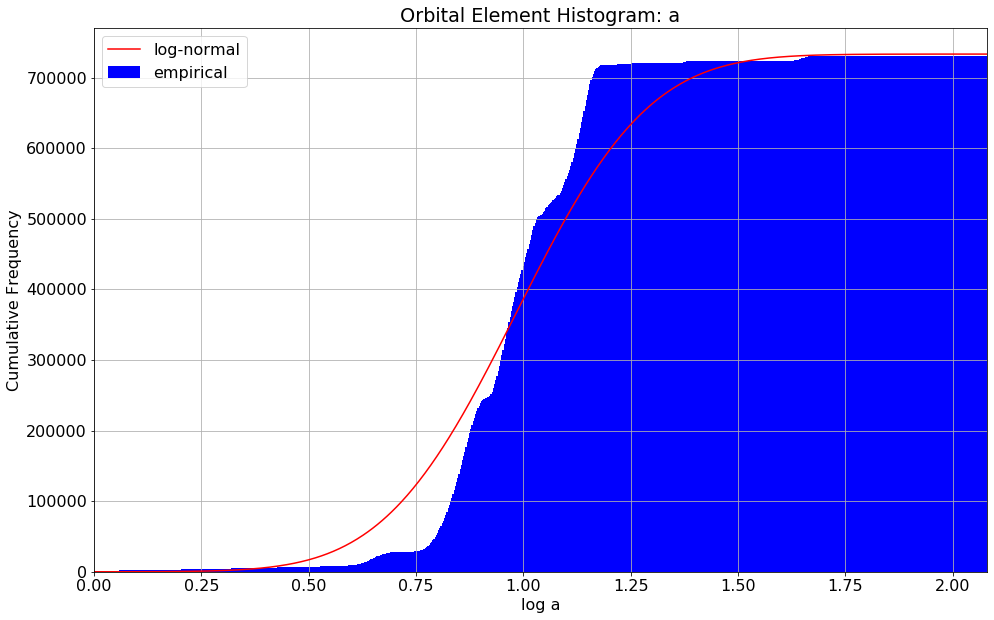
\includegraphics[width=1.0\textwidth]{../figs/elts/elt_hist_a_cdf.png}
\end{center}
\caption[PDF and CDF for $\log(a)$, Log of the Semi-Major Axis.]
{PDF and CDF for $\log(a)$, Log of the Semi-Major Axis.\\
We can clearly see the famous \href{https://en.wikipedia.org/wiki/Kirkwood_gap}{Kirkwood gaps} in the PDF. \\
The CDF shows that on a macroscopic scale, a log-normal model isn't bad.\\
$\log(a)$ is sampled empirically from the CDF.}
\label{fig:elt_dist_a}
\end{figure}
\clearpage

\begin{figure}[hbt!]
\begin{center}
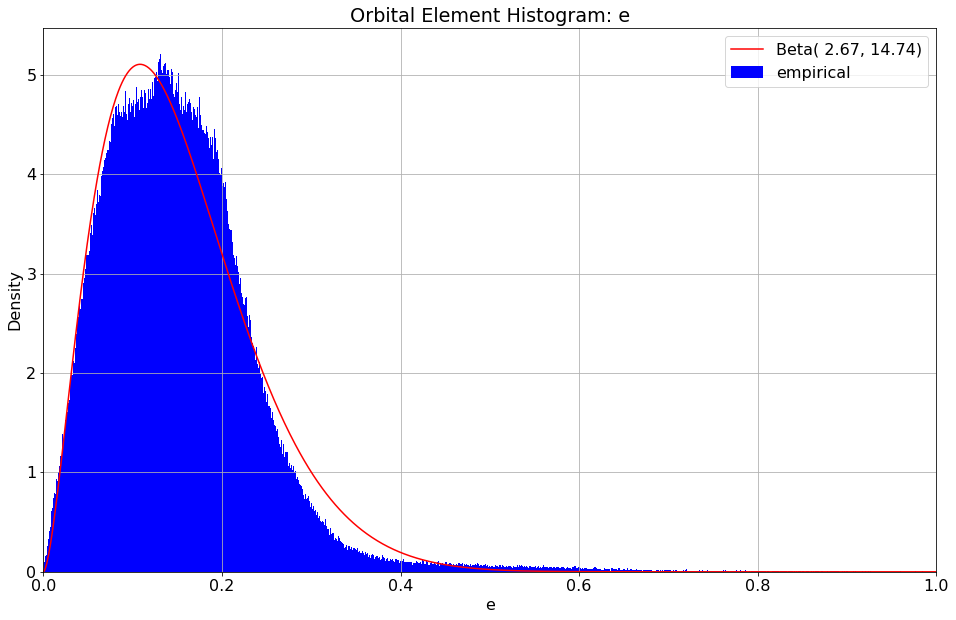
\includegraphics[width=1.0\textwidth]{../figs/elts/elt_hist_e.png}
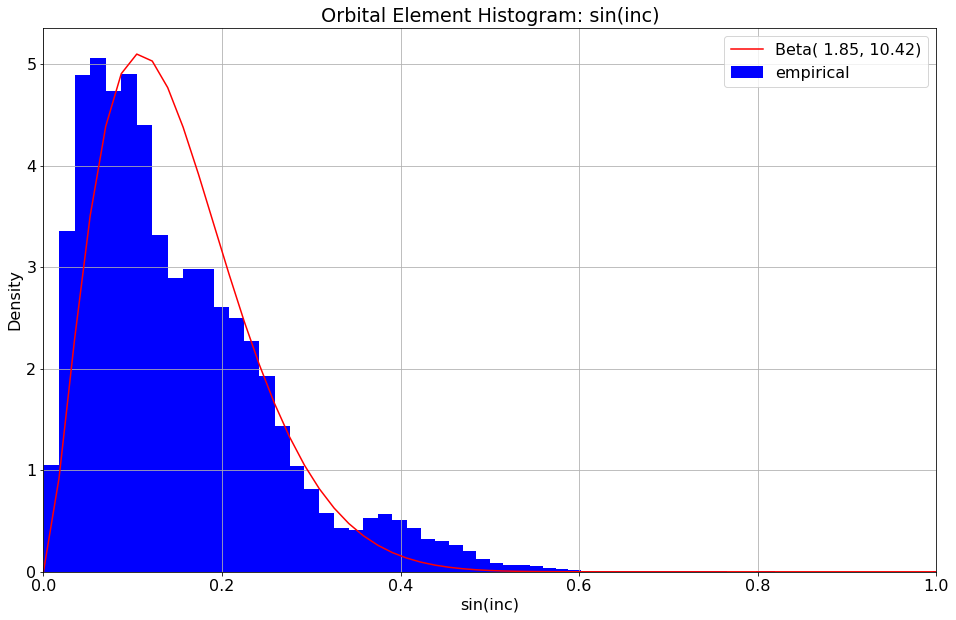
\includegraphics[width=1.0\textwidth]{../figs/elts/elt_hist_i.png}
\end{center}
\caption[PDF for Eccentricity $e$ and $\sin(i)$ (Sine of the Inclination).]
{PDF for Eccentricity $e$ and $\sin(i)$ (Sine of the Inclination).\\
Both $e$ and $\sin(i)$ are bounded in $[0, 1]$ and can be decently approximated by a Beta distribution.\\
Both $e$ and $i$ are sampled empirically from the CDF; Beta sampling could have also worked well.}
\label{fig:elt_dist_e_i}
\end{figure}
\clearpage

\begin{figure}[hbt!]
\begin{center}
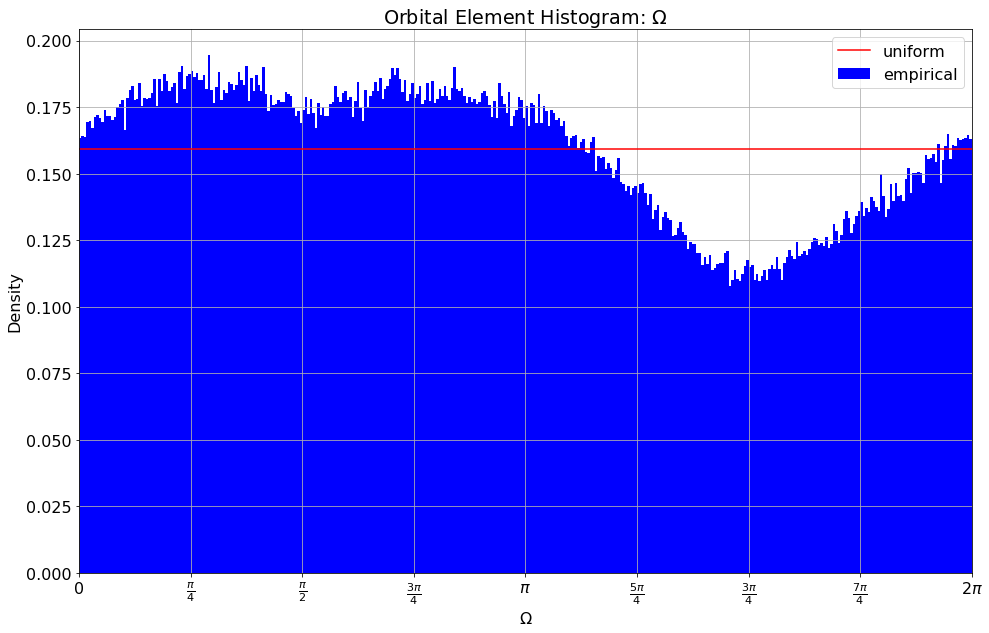
\includegraphics[width=0.95\textwidth]{../figs/elts/elt_hist_Omega_node.png}
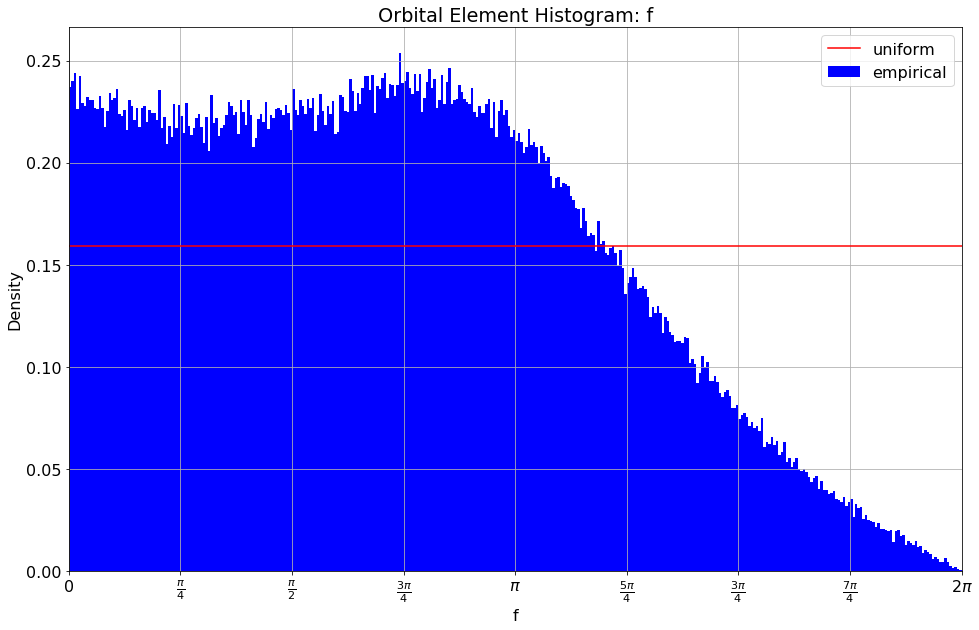
\includegraphics[width=0.95\textwidth]{../figs/elts/elt_hist_f.png}
\end{center}
\caption[PDF for Longitude of Ascending Node $\Omega$ and True Anomaly $f$]
{PDF for Longitude of Ascending Node $\Omega$ and True Anomaly $f$.\\ 
The PDF for $\Omega$ is somewhat close to uniform, but with a noticeable departure.\\
The PDF for $f$ has an odd shape that I would have been hard pressed to predict ahead of time.\\
$\Omega$ is sampled empirically from the CDF; $f$ is computed by sampling $M$ uniformly.}
\label{fig:elt_dist_Omega_f}
\end{figure}
\clearpage

\begin{figure}[hbt!]
\begin{center}
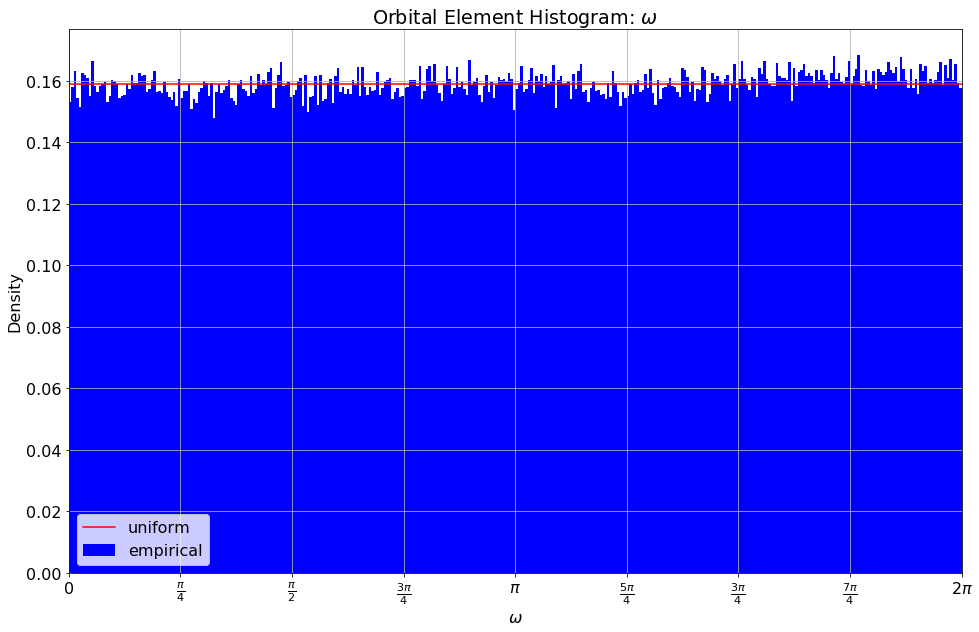
\includegraphics[width=1.0\textwidth]{../figs/elts/elt_hist_omega_peri.png}
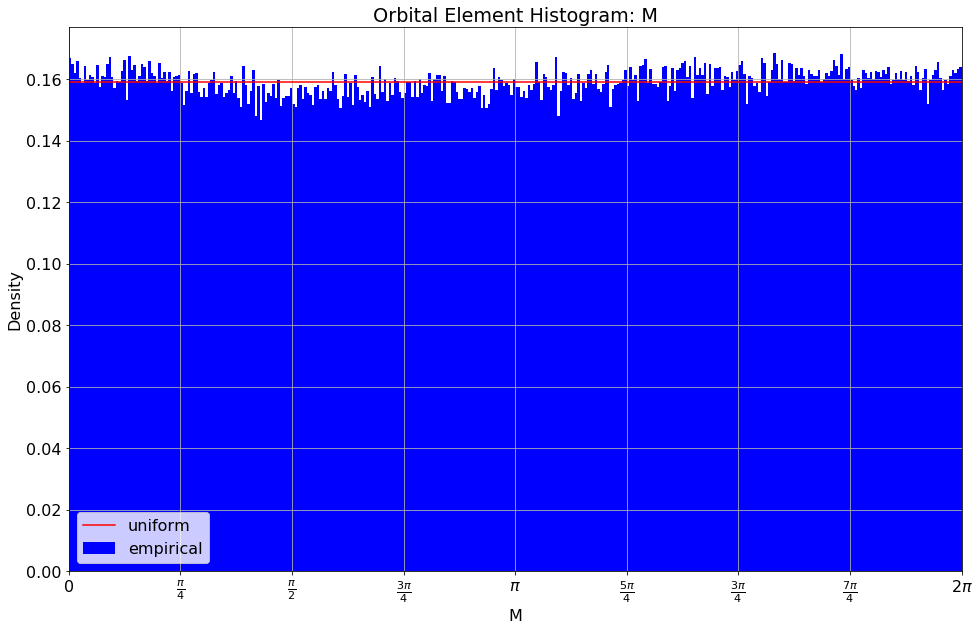
\includegraphics[width=1.0\textwidth]{../figs/elts/elt_hist_M.png}
\end{center}
\caption[PDF for Argument of Perihelion $\omega$ and Mean Anomaly $M$]
{PDF for Argument of Perihelion $\omega$ and Mean Anomaly $M$.\\ 
As promised, these are empirically very close to the uniform distribution we would expect.\\
Both of these elements are sampled uniformly at random.}
\end{figure}
\clearpage

If a continuous rather than discrete sampling strategy were desired, $e$ and $\sin(i)$ could be well approximated by 
a fitted Beta distribution as shown in the preceding charts. 
% this approach, though, would tend to undersample high eccentricity candidates.
Drawing $\log(a)$ from a theoretical distribution could be a bit messy.  
To my eye, the best solution there would be a mixture of normals with perhaps $6$ to $10$ components.
I see little argument in favor of drawing $a$ or $\omega$ other than empirically.
Random elements are generated in the module \tty{candidate\_elements.py} with the function \tty{random\_elts}.
A random seed is used for reproducible results.

\section{Assembling ZTF Detections Near Candidate Elements}
\label{section_ztf_elements}
Once we've generated a set of candidate orbital elements, 
the next step in the computation is to find all the ZTF detections that lie within a given threshold of the elements.
We've already introduced the important ideas that go into this computation in earlier sections.
The only difference is that instead of calculating the direction of a known asteroid whose orbit was integrated and saved to disk, 
we integrate the orbit of the desired elements on the fly.
Then we proceed to calculate the predicted direction from the Palomar observatory and filter down to only those within the threshold
(I used 2.0 degrees in the large scale search.)

The module \tty{ztf\_element} includes a function \tty{load\_ztf\_batch} that takes as arguments dataframes \tty{elts} and \tty{ztf}
of candidate orbital elements and ZTF observations to cross reference against.
It also takes a threshold in degrees.
It returns a data frame of ZTF elements that is keyed by \tty{(element\_id, ztf\_id)}
where \tty{element\_id} is an identifier for one candidate element (intended to be unique across different batches)
and \tty{ztf\_id} is the identifier assigned to each ZTF detection.

The work of integrating the candidate elements on a daily schedule is carried out by \tty{calc\_ast\_data} in module \tty{asteroid\_dataframe}.
The work of splining the daily integrated asteroid positions and velocities at the distinct observation times is done in \tty{make\_ztf\_near\_elt}.
Because this computation is fairly expensive (it takes about 25 seconds to integrate a batch of 64 candidate elements),
a hash of the inputs is taken and the results are saved to disk using the hashed ID.
If a subsequent call for the ZTF elements is made with the same elements, it is loaded from the cache on disk.

Those readers who would like an interactive demonstration can find one in the Jupyter notebook \tty{06\_ztf\_element.ipynb}.
Figure ~\ref{fig:ztf_elt_dataframe} shows a preview of the output dataframe \tty{ztf\_elt}:
\begin{figure}[hbt!]
\begin{center}
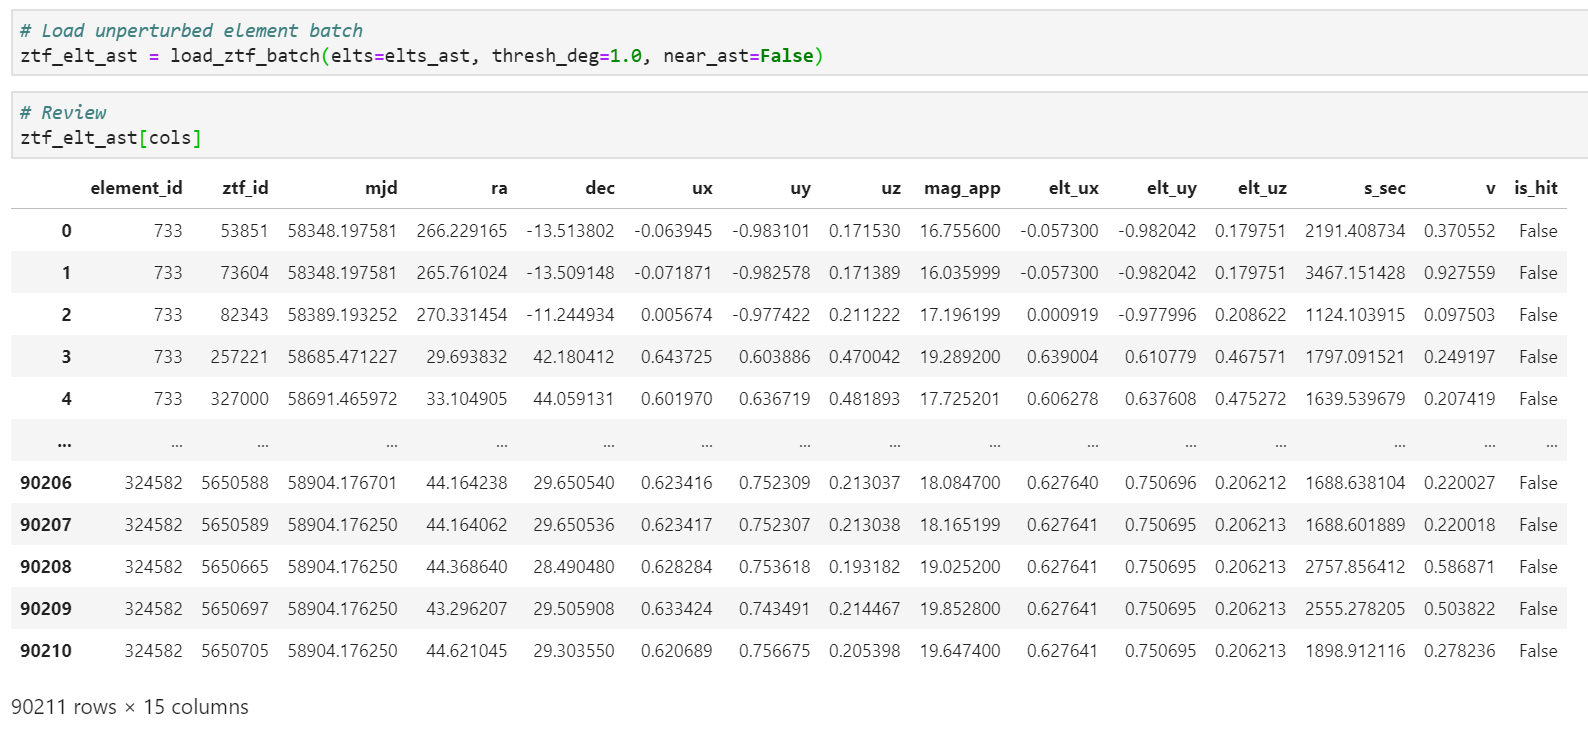
\includegraphics[width=1.0\textwidth]{../figs/elts/ztf_elt_dataframe.png}
\end{center}
\caption[ZTF Detections Within a 1.0 Degree Threshold of a Batch of 64 Orbital Elements]
{ZTF Detections Within a 1.0 Degree Threshold of a Batch of 64 Orbital Elements.}
\label{fig:ztf_elt_dataframe}
\end{figure}
In Chapter 3, we showed that the quantity $v = (s/\tau)^2$ is would be distributed $\sim \Unif[0,1]$
if predicted distributions were distributed uniformly at random.
The function \tty{plot\_v} in module \tty{element\_eda} generates such a plot.
I generated a list of the 64 asteroids that have the most hits in the ZTF dataset (ranging from 148 to 194).
Then I generated ZTF dataframes for three collections of orbital elements: 
\begin{itemize}
\item unperturbed orbital elements belonging to these 64 asteroids
\item perturbed orbital elements of these 64 asteroids
\item random orbital elements
\end{itemize}
As a test of the theory and to build intuition, Figure ~\ref{fig:candidate_elt_v} plots the distribution of $v$ 
against a threshold of 1.0 degree for these three sets of candidate elements.
The results are exactly as predicted.
The random distribution is approximately uniform as expected.
The unperturbed distribution is a mixture of uniform and a spike in the first bucket.
The perturbed distribution is in between, with the hits leaking out over the first few buckets out to $v \approx 0.07$ (about 250 arc seconds).
\begin{figure}[hbt!]
\begin{center}
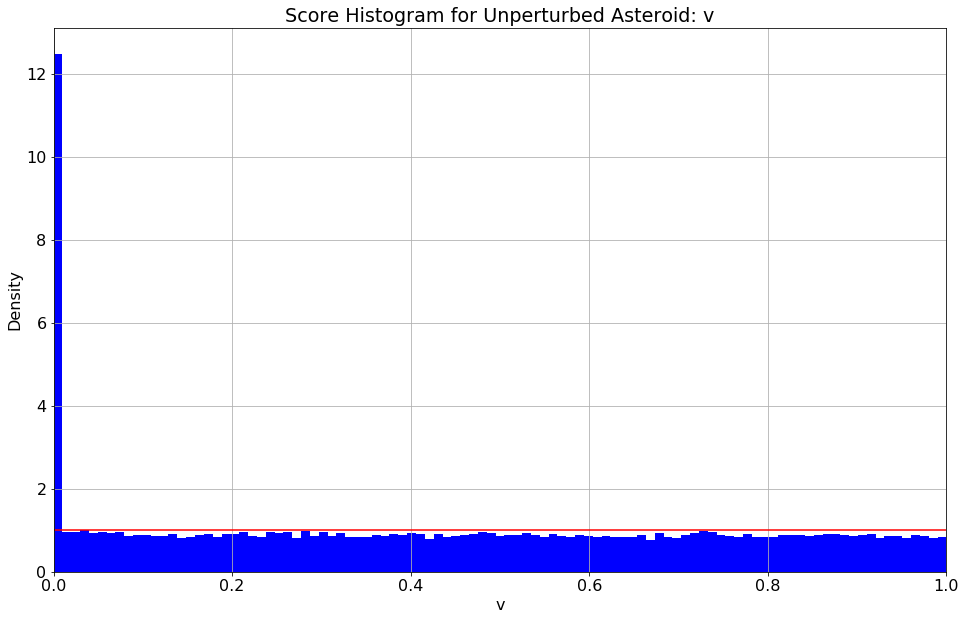
\includegraphics[width=0.70\textwidth]{../figs/elts/v_hist_unperturbed.png}
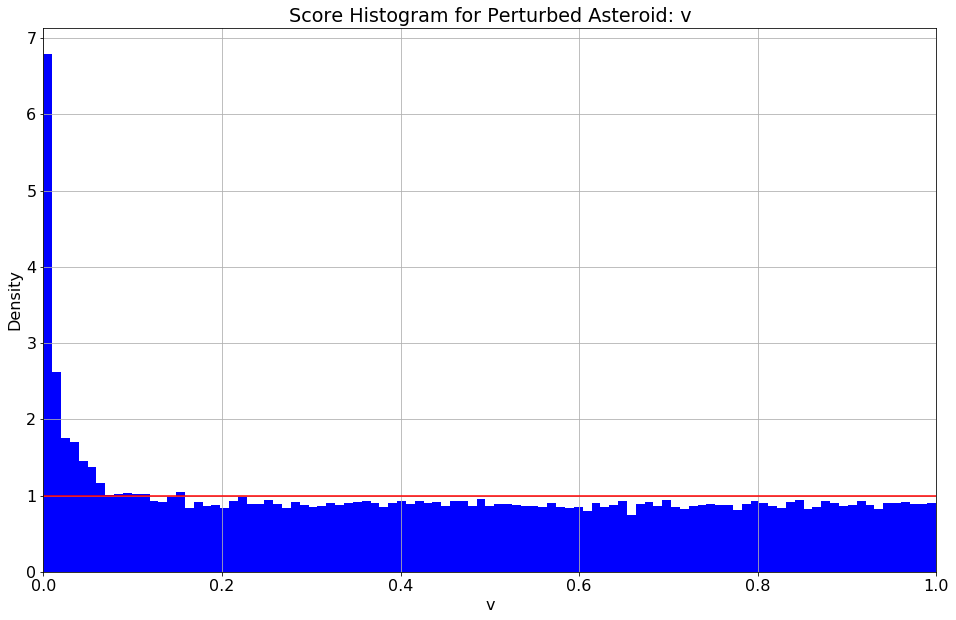
\includegraphics[width=0.70\textwidth]{../figs/elts/v_hist_perturbed.png}
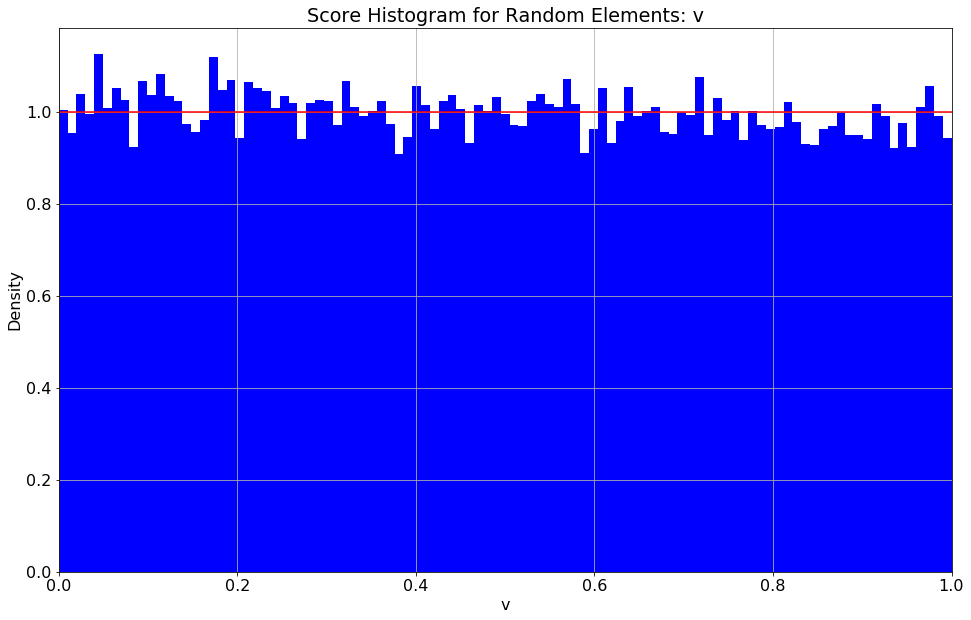
\includegraphics[width=0.70\textwidth]{../figs/elts/v_hist_random.png}
\end{center}
\caption[Histogram of $v = (s/\tau)^2$ for Three Sets of Candidate Orbital Elements]
{Histogram of $v = (s/\tau)^2$ for Three Sets of Candidate Orbital Elements.}
\label{fig:candidate_elt_v}
\end{figure}
\clearpage

\section{Filtering the Best Random Elements}
\label{section_best_random_elements}
One idea is to perform a preliminary screening of the candidate orbital elements 
before investing a large amount of computational resources into running an asteroid search on them.
In the next section we will show how to generate the ZTF detections within a threshold $\tau$ of the candidate elements.
We've already seen that the random variable $V = (S/ \tau)^2$ is distributed $V \sim \Unif(0, 1)$.
We can assess candidate elements by taking the sample mean of $\log(v)$;
we want to explore elements that have a disproportionate share of hits where $v$ is small.
Here is a quick demonstration that for $V \sim \Unif(0,1)$, $\log(V)$ has expectation $-1$ and variance $1$.
\begin{align*}
\E[ V ] &= \int_{v=0}^{\infty} \log (v) dv = \left. v \log v - v \right]_{0}^{1} = (1 \cdot \log 1 - 1) - (0 - 0) = -1 \\
\Var[V ] &= \E[V^2] - \E[V]^2 = \int_{v=0}^{1} \log(v)^2 dv - (-1)^2 \\
&= \left. v \cdot (\log v)^2 - 2 \log v + 2) \right]_{0}^{1} = 2 -1 = 1
\end{align*}
If a set of candidate elements has $n$ detections within threshold $\tau$ with relative squared distances of $v_1, \ldots v_n$,
their sample mean $\bar{v}$ will have expectation $-1$ and variance $n$, so I construct a t-score for candidate elements
$$T = \frac{-(\bar{v} + 1)}{n}$$
This score would be distributed $T \sim \mathcal{N}(0, 1)$ (standard normal) if the guessed positions were uniformly random.
It provides a computationally efficient way to screen candidate orbital elements.

This screening is performed in the module \tty{random\_elements}.
The function \\
\tty{calc\_best\_random\_elts} generates a large batch of random elements (the default size is 1024).
It then builds the ZTF observations close to them and extracts the t-score as described above.
The input batch size is used to select that many of the candidates that have the best score.
The whole process of building the ZTF data frames, searching for the best elements,
and saving the best elements and assembled ZTF data frames to disk is carried out by a Python program that can be run from the command line as
\begin{lstlisting}[style=CodeSnippet]
(kepler) $ python random_elements.py -seed0 0 -seed1 1024 -stride 4 
> -batch_size_init 1024 -batch_size 64 -known_ast
\end{lstlisting}
The example call above runs the program on 256 batches of random elements, with random seeds $[0, 4, \ldots, 1020]$.
The stride argument is to facilitate parallel processing.
The two batch size arguments request that $1024$ initial elements be winnowed down to $64$ with the highest t-scores.
The flag \tty{-known\_ast} at the end asks that only the subset of ZTF detections within 2.0 arc seconds of a known asteroid be used 
to generate the ZTF dataframe and score the initial elements.
I call this searching against known asteroids.
If \tty{known\_ast} is not passed, the behavior is the opposite; only the ZTF detections at least 2.0 arc seconds (i.e. ones that don't closely match) are considered.
I ran this program to generate 4096 candidate elements for each of the known and unknown asteroids.
Altogether it took quite a while to run, over one day of total computer time.
The vast bulk of that time is spent building the ZTF dataframe of detections near the elements.

\section{Formulating the Log Likelihood Objective Function}
\label{section_log_likelihood}
The actual asteroid search is an optimization performed in TensorFlow using gradient descent.
Perhaps the most important choice is that of the objective function.
Qualitatively we know that we want an objective function that will be large when we are very close 
(within a handful of arc seconds) to some of the detections.
We don't have a preference about the distance to the other detections.
While it might seem tempting to write down an objective that rewards being close to everything, that's not at all what we want.
Such an objective function would encourage us to find some kind of ``average orbital element'' for all the asteroid detections  in this collection.
But we want to find the elements of just one real asteroid.

A principled way to formulate an objective function is with probability.
As a reminder, $S$ is the Cartesian distance between $\upred$ and $\uobs$,
and $\tau$ is the threshold Cartesian distance so only observations with $S < \tau$ are considered.
$V = (S / \tau)^{2}$ is in the interval $[0, 1]$.
Introduce the following probability mixture model for the random variable $V$.
Some unknown fraction $h$ (for hits) of the observations are associated with one real asteroid, whose elements we are converging on.
Conditional on an observation being in this category (a hit), the distribution of $V$ is exponential with parameter $\lambda$.
Conditional on an observation being a miss, $V$ is distributed uniformly on $[0,1]$.
In the formalism of conditional probability,
\begin{align*}
V | \textrm{Hit} &\sim \Expo(\lambda) \\
V | \textrm{Miss} &\sim \Unif(0,1)
\end{align*}
We can relate the parameter $\lambda$ to a resolution parameter $R$ by observing that $v=(s/\tau)^2$ and
$$f(v) \propto e^{-\lambda v} = e^{-\lambda s^2 / \tau^2}$$
This looks just like a normal distribution in the Cartesian distance $s$, a plausible and intuitive result!
Let us identify the standard deviation parameter $\sigma$ of this normal distribution with the resolution $R$,
i.e. think of the PDF $f(s)$ as being normal with PDF $f(x) \propto e^{-s^2 / 2 R^2}$.\\
Equating the exponent in both expressions, we get the relationship
$$ \lambda = \frac{\tau^2}{2R^2}$$

It is convenient to use $\lambda$ for calculations, both mathematical and in the code.
For understanding what is going on, I find it more intuitive to use the resolution, since it's on the same scale as the threshold $\tau$.
The PDF of an exponential distribution is given by \cite{BH}
$$ f(v; \lambda) =\lambda e^{-\lambda v}$$
In this case, we need to modify this PDF to account for the fact that $v \in [0,1]$ 
while the support of the exponential distribution is $[0, \infty)$.
What we want instead is the truncated exponential distribution, which is normalized to have probability $1$ on the interval $[0,1]$, namely
$$ f(v| \mathrm{Hit}, \lambda) = \frac{\lambda v}{1 - e^{-\lambda}}$$
Of course, the PDF of the uniform distribution is just $1$, so
$$ f(v | \mathrm{Miss}) = 1$$
Now we can write the PDF of the mixture model using the Law of Total Probability:
\begin{align*}
f(v| h, \lambda) &= f(v|\mathrm{Hit}, \lambda) \cdot P(\mathrm{Hit}) + f(v|\mathrm{Miss}) \cdot P(\mathrm{Miss}) \\
&= h \cdot \frac{\lambda v}{1 - e^{-\lambda}} + (1 - h)
\end{align*}

The optimization objective function will be the log likelihood of the PDF:
$$ \mathcal{L}(\vvec, h, \lambda) = \sum_{j=1}^{n} \log \left( h_j \cdot \frac{\lambda v_j}{1 - e^{-\lambda_j}} + 1 - h_j \right)$$
Please note that I've omitted the parameter $\tau$ from these expressions to lighten the notation.
During the training of the model, the $\tau$ parameter is also updated.
The three mixture parameters that are manipulated during training are 
\begin{itemize}
\item $N_h$: the number of hits for this candidate element
\item $R$: the resolution of this candidate element as a Cartesian distance
\item $\tau$: the threshold of this candidate element as a Cartesian distance
\end{itemize}
The hit rate $h$ is computed from $N_h$ by dividing by the number of rows that are within the threshold distance.
The dimensionless error term $v$ is computed by taking $v = (s/\tau)^2$.
The exponential decay parameter $\lambda$ is calculated as $\lambda = \tau^2 / 2R^2$.

In general, a likelihood function is only defined up to a multiplicative factor and a log likelihood up to an additive constant.
In a theoretical analysis of maximum likelihood, the constant is typically irrelevant because one is differentiating the likelihood function anyway.
In this problem, I want to set the constant term so that a log likelihood of zero equates to having no information,
i.e. an uninformative baseline.
This is particularly easy to do here: if we set $h=0$, the terms involving the truncated exponential distribution all drop out 
and the log likelihood becomes a sum of $\log(f) = \log(1) = 0$.
In general, we can zero out the log likelihood function by evaluating it at a set of uninformative baseline values, 
and subtracting this quantity $\mathcal{L}_0$ (the baseline likelihood) from the current optimized $\mathcal{L}$.

There is an important intuition about the role of the mixture parameters that I would like to explain.
The major challenge in tuning the resolution $R$ is for the gradients to encourage the model to adjust the orbital elements
to get closer to detections that are likely to be hits, without getting deked 
\footnote{\href{https://en.wikipedia.org/wiki/Deke_(ice_hockey)}{deke}: an ice hockey technique whereby a player draws an opposing player out of position.\\
It is a Canadian contraction of the word ``decoyed'.'}
by close-ish detections that belong to other asteroids.
If the resolution parameter $R$ is too small (sharp focus) before convergence, the model will be too far away to pick up any gradient to the hits.
It will achieve a negative log likelihood because $\log(1-h) < 0$ and it won't make it up from the putative hits.
If $R$ is too high (fuzzy), the model will end up compromising and trying to fit a cloud of detections belonging to different asteroids.
The whole game of getting the model to converge is to find the sweet spot of $h$ and $R$ where the model gradually tightens its focus,
like letting your foot off the clutch when you put a car with a manual transmission \footnote{Otherwise known as a real car} into gear. 

In previous iterations, I attempted to write down objective functions to balance these objectives by hand and failed miserably.
It was only when I used probability theory with a mixture model that plausibly describes the underlying facts that I had any success.

The likelihood function above applies to only one of the candidate orbital elements.
In the actual optimization of a batch of 64 elements, we need a single scalar valued objective function.
Because all of the elements in a batch are being optimized independently and have no interaction with each other, we can simply take their sum.
There is an important refinement to this idea, though, that I will discuss in section ~\ref{section_asteroid_search}.

\subsection{Adding the Magnitude to the Joint Likelihood Function}
The likelihood function written above depends only on the probability distribution of the squared relative distance $v = (s/\tau)^2$.
A more sophisticated model will also predict the magnitude.
We can write down a simple probability density for the magnitude as well by assuming that it is normally distributed.
We can treat $H$ and $\sigma_{mag}$ as learnable parameters, analogous to a learned ``orbital element'' for the the absolute magnitude $H$
and a learned ``resolution'' for apparent magnitude.
A strong argument can be made that the magnitude errors are independent of the direction errors, 
so the joint PDF $f(v, h) = f_{v}(v) \cdot f_h(h)$.
The PDF $f_h(m)$ will be $\varphi( (m - H) / \sigma_H) / \sigma_h$ where $\varphi(z)$ is the standard normal PDF.

This time, we will need to specify the alternate, uninformed baseline, because it isn't just 1 as is the case for the uniform distribution on $[0,1]$.
This can be done by taking the sample mean and variance of all the observations within the current threshold $\tau$;
this calculation yields the term $\mathcal{L}_0$ discussed above.

I tried all of this, and got it working somewhat, enough that the model could function.
But I found that my predictions of the magnitude were too finicky, enough so that the model performed better when 
I set the objective function as the simple log likelihood depending only on the angular distance.
The code is present in \tty{AsteroidSearch} and \tty{TrajectoryScore} to incorporate the magnitude 
into the likelihood in the future if the prediction can be tightened up enough to work.

\section{Performing the Asteroid Search}
\label{section_asteroid_search}
We have by now covered the main theoretical ideas that go into the asteroid search.
We've seen how to generate a set of candidate orbital elements and a collection of ZTF observations within a threshold of these elements.
And we've identified a log likelihood function that rewards orbital elements for getting close to detections likely to be real 
while learning mixture parameters to describe the provenance of observations under consideration and how closely they have been fit.
In this section I will explain some of the most important details that were required to get this model to actually learn orbital elements from data.

The workhorse class that searches for asteroids is called \tty{AsteroidSearchModel}.  
It's a Keras custom model defined in the module \tty{asteroid\_search\_model.py}.
An \tty{AsteroidSearchModel} is initialized with a batch of candidate elements and the ZTF observations near these elements.
It constructs two layers of type \tty{CandidateElements} and \tty{MixtureParameters} that maintain, respectively, 
the candidate orbital elements and mixture parameters.
These layers are defined in the module \tty{asteroid\_search\_layers.py}.
The candidate orbital elements are the familiar seven Keplerian orbital elements.
The six ``live'' ones $(a, e, i, \Omega, \omega, f)$ are trainable variables, and the epoch is locked at its initial value.
The mixture parameters are $N_h$, $R$ and $\tau$, all of which are trainable.

\subsection{Controlling Parameters on a Uniform Scale}
The first important idea in training the model is that all variables are controlled internally 
with TensorFlow variables that are scaled with a comparable range, almost always $[0, 1]$.
For example, the orbital element $a$ in the candidate elements layer is controlled by a \tty{tf.Variable}
named \tty{a\_} that is constrained to lie in the region $[0, 1]$.
(If a gradient update tries to push it less than 0 or more than 1, it is clipped back in the allowed range.)
The value of $a$ is computed on demand by
$a = a_{\mathrm{min}} \cdot \exp( \tty{a\_} \cdot \tty{log\_a\_range})$ 
where \tty{log\_a\_range} = $\log(a_{\mathrm{max}} / a_{\mathrm{min}})$.\\
$a_{\mathrm{min}}$ and $a_{\mathrm{max}}$ are set by policy to 0.5 and 32.0, respectively.
Other orbital elements are likewise controlled via mathematical transforms into the range $[0, 1]$.
The eccentricity is left as is, though it is limited to at most $63 / 64 = 0.984375$ to avoid numerical instabilities that occur as $e$ approaches $1$.
The inclination is controlled via $\sin(i)$, which is constrained to lie in the interval $\pm 1 - 2^{-8}$.
The other angle variables $\Omega$, $\omega$ and $f$ are unconstrained, but multiplied by $2 \pi$ 
so the control variable $f\_$ for instance can cover its entire allowed range of values by moving 1.0.

The number of hits \tty{num\_hits} is allowed in a range of $6$ to $1024$ and controlled by its log.
I set the minimum to $6$ because any smaller than that, there is no point to searching at all.
The resolution is controlled on a log scale as well and allowed in a range of 1.0 to 3600 arc seconds.
The threshold is controlled on a log scale and allowed in a range of 10.0 arc seconds 
up to the original threshold used to assemble the data, which is 7200 arc seconds in my runs.

What is the point of these machinations?
It might be obscure to readers with a background in astronomy or applied math, but machine learning practitioners should be less surprised.
Scaling variables to have a common size is a basic technique that significantly aids gradient descent in practice.

\subsection{Gradient Clipping by Norm}
A second important technique for the optimization is gradient clipping.
The objective function is optimized using the de facto default in TensorFlow, Adam (adaptive moments).
Gradient clipping is not turned on by default, but I found it to be vital for this problem to work.
The reason it's so important is that the optimization function (and its gradients) vary over a tremendous scale in this problem.
At the start of training, there is little to no information; the likelihood function is near zero; and the gradients are relatively small.
As the model reaches convergence if it is lucky enough, it can achieve significantly large likelihoods and huge gradients.
All gradients are clipped by norm to a maximum norm of 1.
A good intuition for gradient clipping by norm is that the direction of the gradient is not changed, but the magnitude is capped.
My sense from training the model extensively is that the gradient is almost always ``saturated'' 
(i.e. the original gradient has a norm larger than 1, which is reduced to 1 by the gradient clipping.)

The combination of having all the control variables in a range $[0, 1]$ and gradients clipped at a norm of $1$
gives us a useful intuition about how quickly the model can update its parameters.
I perform training in ``joint mode'' (where both the orbital elements and mixture parameters are updated) with a learning rate of $2^{-16}$.  
This is a factor of 64 smaller than the Adam default of 0.001, which I found to be far too high for this problem.
Pretend for a moment that there were only 1 parameter.  
Assuming the gradient is saturated, on each data sample encountered, it will either increase or decrease by the learning rate.
So after encountering $2^{16} = 65,536$ samples it would be able to move from one extreme of its values to another.
Of course in practice with multiple parameters, a single parameter will almost never have a partial gradient equal to 1.0,
but it's a good intuition for the ``speed limit'' of how fast any one parameter can change during training.

\subsection{Scoring Trajectories: Log Likelihood and Hits by Candidate Element}
Let's now sketch out the flow of information from the candidate elements and mixture parameters all the way to the objective function.
When the model is initialized, it also constructs an \tty{AsteroidDirection} layer.
We've discussed this before--it's the layer that computes a Kepler orbit from the current candidate orbital elements,
including a calibration adjustment that is periodically updated by numerically integrating the current candidate elements.
The important thing to remember is that the asteroid direction layer is predicting directions based on candidate orbital element tensors
that are the output of the candidate\_elements layer.

Now a new layer comes into play: the \tty{TrajectoryScore} layer.
This layer is also defined in \tty{asteroid\_search\_layers}.
When the model is initialized, this layer saves the directions of all the observations in the ZTF data frame as Keras backend constants.
This was a deliberate design choice that is somewhat unorthodox.
Keras models are largely designed around the assumption that during training you will feed in batches with equal numbers of input and output samples.
This problem has a quite different flavor.
There are no ``outputs'' we can line up against a batch of 64 candidate orbital elements.
And the only ``inputs'' are the initial candidate orbital elements, which are trainable variables.
Eventually I needed to pass a dummy input that had \tty{batch\_size} ones in it to placate Keras.

We are just computing an objective function and trying to maximize it, using TensorFlow as a big computational back end with
support for GPU computation, automatic differentiation, and gradient descent optimization.
By putting all the observations into Keras constants, we write them to the GPU once when the model is initialized,
and then there is no need to copy any data between CPU and GPU memory during training.
Eventually I can imagine training this model on such a huge data set that it might be necessary to batch the observation data.
But with modern GPUs having memory capacities on the order of 10 GB, I think this approach should scale very well and offers significant performance benefits.

The trajectory score layer is passed a tensor with the predicted directions $\upred$ as well as the current mixture parameters.
It computes the Cartesian difference $s$ between the predicted and observed directions, 
then applies the current filter $\tau$ to assemble a new tensor $v$ of the relative distance squared in $[0,1]$.
All of these tensors should be thought of as having a shape starting with the batch size;
$s$ for instance is one long tensor that represents the distances for all 64 orbital elements, concatenated together.
The trajectory score layer then goes through the calculation of the probability and log likelihood under the mixture model described above.
It returns a tensor of log likelihoods, one log likelihood for each of the 64 candidate orbital elements.
It also counts the number of hits, which are defined here as observations that are within 10.0 arc seconds of their predicted directions.

\subsection{Training Each Candidate Element Independently}
During my early efforts to train this model, I struggled to find a learning rate that worked.
I found that different elements converged at different times and had very different gradients.
In my intuition, I want to pretend that the gradient has only six terms for the candidate elements and three terms for the mixture parameters.
When the gradient is clipped to a size of 1 across a row, 
it's helpfully giving us a direction that we should adjust the elements and mixture parameters for that candidate element.
But what TensorFlow is really doing is squashing the whole gradient, all 64 candidate elements worth, to have a norm of 1.
When one element has a large gradient, it will dominate at the expense of the others.

In writing this out now, I realize that what I probably should have done was to write a custom gradient clipping class that works on one candidate element at a time.
What I did instead was to reason that I wanted the ability to effectively tune the learning rate on all 64 of the candidate elements independently.
Of course a model of this kind has only one scalar objective function and one learning rate.
But we can achieve the same effect by weighting the contribution of each candidate element.
If $\mathcal{L}_i$ is the log likelihood of the $i$th candidate element, and $w_i$ is the weight on the $i$th candidate element,  
then the weighted objective function is 
$$\mathcal{L} = \sum_{i=1}^{b} w_i \mathcal{L}_i$$
The weights are initialized at $w_i=1$.  If we cut the weight $w_2$ to $0.5$, then all the gradients due to candidate element $2$ will also be cut in half.

But how do we decide when to adjust the weights?
One problem I ran into repeatedly was the model would make quite good progress, 
then it would get to a region where the learning rate was too high and in just one epoch it would fall apart.
I tried to alleviate this using the built in early stopping, but this doesn't stop in time to recover when the training goes bad this fast.
And even if it did, it only knows about the single, scalar valued loss function;
it has no notion that out of 64 elements, 56 improved on the last epoch but 8 got worse and so should be rolled back.
I ended up writing my own custom code to do exactly this.
At the end of a series of epochs of training, which I refer to as one ``episode'' of adaptive training,
I check which elements have regressed and have worse log likelihoods than before.
Any element that has regressed has its candidate elements and mixture parameters rolled back to their prior (best) values.
Those elements also have their weights adjusted by a factor of 0.5, i.e. they are cut in half.
I call this procedure ``adaptive training'' because the learning rate is adaptive.
I found that this simple idea significantly improved the performance of the training.
Without it, I was forced to use glacially slow learning rates to avoid overshooting and collapse (I even tried $2^{-20}$ in one bleak moment of desperation).

\subsection{Training in ``Mixture'' and ``Joint'' Modes}
The first test I tried was to give the model a set of candidate orbital elements that exactly 
matched the 64 asteroids with the most observations in the data set (around 160 each on average).
I figured that this problem would be a piece of cake for the model.
It would pick up close to zero gradients on the orbital elements, and a huge gradient by tightening the resolution,
and focus in tighter until it converged, right?
Wrong! The problem is that when the resolution and threshold distances are too large, 
the model is attaching a lot of weight to observations that are far away.
The early iterations polluted the good orbital elements and it never managed to converge.

I hit on the idea of freezing the candidate orbital elements and only training the mixture parameters.
Of course, this feels a bit like cheating.  
If you know the elements are right and just want to learn the mixture parameters, 
of course you're going to do better if you freeze the elements and only train the mixture parameters.
At first, this was only a testing technique.
Later on, though, I realized that it helps the model to converge even when it's not cheating.
My intuition is that it's ``safer'' to train the model at a higher learning rate when you adjust 
the mixture parameters than when you adjust the candidate elements as well.

The model as it now stands alternates rounds of training in two modes: ``mixture'' and ``joint'' modes.
In mixture mode, only the mixture parameters $N_h$, $R$ and $\tau$ are trainable.
The learning rate is higher by a factor of 16, $2^{-12}$ in mixture mode vs. $2^{-16}$ in joint mode.
The most important difference, though, is that the objective function is adjusted.
When I started out, I had only two trainable mixture parameters, $N_h$ and $R$.
I noticed that the model wasn't converging all the way, and realized that I wanted it to reduce $\tau$ along with $R$ as it trained.
This is quite intuitive.  

\subsection{Modifying the Objective Function to Encourage Convergence}
You might start out with observations within 2.0 degrees and a resolution of 0.5 degrees.
But if you've trained to the point of a resolution of 0.1 degrees, there's no reason to drag around observations that are 20x further away.
They're just noise, and they're hampering your ability to fine tune.
I noticed at this point that after I made $\tau$ trainable, the model never wanted to reduce it.
In hindsight this made sense: the likelihood always looks better when you consider it against a larger threshold.
If your parameters are within 50 arc seconds on 100 observations vs. a threshold of 2.0 degrees (7200 arc seconds), 
you're going to pat yourself on the back and say ``that's pretty good, it's not too likely I could have achieved that by chance alone.''
If you shrink the threshold from 2.0 to 1.0, your $v$ is going to quadruple and your log likelihood will plummet.

This suggests that while log likelihood is an excellent objective function for separating ``more likely'' from ``less likely'', it's not exactly what we want here.
Even if the log likelihood has a very strong local maximum at a fully converged solution,
this experience was telling me that there was no smooth path of increasing gradients to get there.
Instead, I wanted an optimization function that would encourage the model to converge.
I modified the objective function to take the more general form
$$J = \sum_{i=1}^{b} w_i \cdot \frac{\mathcal{L}_i}{R_i^\alpha \cdot \tau_i^\beta}$$
This is the same as before, but now there are powers of the resolution $R_i$ and threshold $\tau_i$ in the denominator.
While the original objective function only sought to find the most likely configuration,
this objective function is willing to trade a reduction in likelihood for a more concentrated (converged) prediction.
It's effectively adjusting the scoring for the ``degree of difficulty'' like Olympic diving and gymnastics.
It's harder to generate orbital elements and mixture parameters with a resolution of 10 arc seconds against a threshold of 40 arc seconds
than to do it with the initial settings of 0.5 and 2.0 degrees respectively.

I would also like to quickly state a theoretical motivation for this formulation, which originally motivated it.
Going back to the idea that we have random variables $V_1, \ldots V_n \iid \Unif(0, 1)$,
we saw that the quantity $T = n^{-3/2} \cdot \sum_{i=1}^{n} \sim \mathcal{N}(0,1)$ had the same distribution regardless of $n$.
(We divide the sum by $n$ to get the sample mean and by $\sqrt{n}$ to give it variance 1).
Of course, the number of detections $n$ within a threshold $\tau$ is a discrete number, 
so it will have a derivative of zero except at points where it is not defined.
But in the baseline case where we have a uniform density of detections on the sphere,
the expected number of detections within the threshold $\E[n] \propto \tau^2$.
This provides a strong intuition that the log likelihood over $\tau^3$ is a meaningful quantity
and that dividing by a power of $\tau$ is justified.
In the actual event, I experimented with different configurations and settled on $\alpha=1$ and $\beta=1$.
I wanted to guide the resolution and threshold to smaller values at the same rate.
In practice it didn't make a large difference, but these values seemed to work well.

\subsection{Organizing Training: Batches, Epochs, Episodes, and Sieving Rounds}
Training is organized hierarchically into batches, epochs, episodes, and sieving rounds.
The training batch and epoch are already defined terms in machine learning.
One batch consists of the 64 candidate orbital elements and all of the ZTF observations they are scored against.
The number of batches in an epoch is a parameter I set to 64.
Keras reports training on screen by the epoch, 
and the early stopping will kick in to terminate training early if the loss function gets worse.
The size of 64 was set by experimentation.
Too low and there is excessive overhead from logging progress and so on.
Too high and you lose too much progress from bad training before you cut it short.

One episode is the term I use for a period of adaptive training.
It is implemented with the methods \tty{search\_adaptive} and \tty{train\_one\_episode} in the \tty{AsteroidSearch} class.
At the end of an episode, I save the weights and three quantities of interest for each candidate element:
log likelihood, loss function, and number of hits at 10 arc seconds.
If any of these figures of merit have gotten worse during the training round,
I deem the training on those elements to have been a failure, revert the weights for those elements back, and cut the weight on these elements by half.
This is equivalent to selectively reducing the learning rate on these elements by half.
I also re-run the numerical calibration of the position model against the \tty{REBOUND} integrated orbit at the current orbital elements at the end of each episode.

Weights and training progress are saved in the method \tty{save\_weights}.
A separate method called \tty{save\_train\_hist} saves data frames as .h5 files with all information required to serialize the model to disk.
The built in methods for serializing Keras models were not working on this custom model, 
and in any case would have necessitated saving a huge amount of redundant data with all the observations as serialized Keras constants.
These custom methods save only the data that changes (e.g. the candidate elements and mixture parameters) plus some calculations used for monitoring progress.
The process of checking elements to see if they have made progress and reverting them if they regressed 
is done in the method \tty{update\_weights}.

I set the length of an episode to at most 4 epochs; an episode ends early if the Keras early stopping callback detects that the overall loss has gotten worse.
I define the effective learning rate to be the average of the element weights $w_i$ multiplied by the global learning rate.
A training episode is terminated early if the effective learning rate drops below a threshold, which defaults to $1/64$ of the original learning rate.

A sieving round is the highest level of training.
It covers at most a set number of samples.
I set the length of a sieving round to 512 batches for mixture and 2048 batches for joint mode.
A sieving round can also end early if the effective learning rate drops below a threshold.
This extra hierarchical level is added to support adjusting a few settings that change only rarely.
These include manually tuning the maximum permitted resolution and threshold, and resetting the weights on all elements to 1 if desired.
The reason one might choose to reset the weights to 1 is that the adaptive training only reduces the learning rate when training overshoots.
Periodically tuning the $w_i$ back to 1 gives them a chance to rebound if the elements have reached a better spot where the faster
learning rate is now feasible.
The sieving round also provides a convenient interface for alternating between joint and mixture mode.
Finally, the sieving round allows customization of the exponents $\alpha$ and $\beta$ applied to the resolution and threshold 
in the denominator of the objective function.
One sieving round is implemented by the method \tty{sieve\_round}.

The method \tty{sieve} implements a preset schedule of sieving rounds.
For maximum maximum thresholds of 7200, 5400, 3600 and 2400 arc seconds, 
it runs first training in mixture mode for 512 batches at a learning rate of $2^{-12}$, 
then training in joint mode for 2048 batches at a learning rate of $2^{-16}$.
Observe that one sieving round in mixture mode is encountering each data point $2^{9} \cdot 2^{6} = 2^{15}$ times.
Multiplying this by a learning rate of $2^{-12}$, a parameter could theoretically cover its full range 8.0 times in one round.
Similarly, a sieving round in joint mode encounters each data point $2^{11} \cdot 2^{6} = 2^{17}$ times.
At a learning rate of $2^{-16}$ an orbital element could cover its full range of values 2.0 times in a single round.
Remember, though, that there are 64 elements in the batch, and this learning rate is shared by all of them.
If we use the rule of thumb that the norm of the gradient will scale with the square root of of the batch size,
we should divide all of these quantities by $\sqrt{64} = 8$.
This tells us that a mixture parameter on one typical candidate element, moving at maximum speed,
might cover 1.0 times its full range of motion in a sieving round in mixture mode.
An orbital element on a typical element in the batch might cover 0.25 times its range of values
in a sieving round in joint mode.
At the end of this initial phase, a final fine tuning training phase is run with larger powers of $\tau$ and $R$ in the denominator.
This is intended to push the model to achieve full convergence on elements where it has discovered enough hits in the first phase.

\section{Conclusion}
There are many other details that go into the computer code that carries out the asteroid search.
\tty{asteroid\_search\_model.py} has over 2400 lines of code, with an additional 770 in \tty{asteroid\_model} and 930 in \tty{asteroid\_search\_layers}.
In the preceding sections, I have endeavored to present the highlight of the search process, with an emphasis on ideas and policy choices.
In the next section, we will apply these methods to an increasingly difficult series of asteroid search tasks and review the results.